\section{Introduction to Trigonometric Functions}\label{sec:intro_trig}

In this section, we will introduce trigonometric functions. We will examine relationships between these functions and will discuss how to evaluate these functions for commonly used inputs. Trigonometric functions are used frequently in calculus and later courses due to the wide range of phenomena that can be modeled by these functions, everything from airflow in our bronchial tubes to earthquake vibrations in a building.

\vskip \baselineskip
\noindent\textbf{\large Trigonometric Definitions}\\

In this section, we will focus on six trigonometric functions: sine, cosine, tangent, cosecant, secant, and cotangent. These functions are all related to each other, and typically mathematicians focus on sine and cosine since the other four functions can all be expressed in terms of sine and cosine. These relationships are:

\begin{itemize}
	\item $\displaystyle \tan{(\theta)} = \frac{\sin{(\theta)}}{\cos{(\theta)}}$
	\item $\displaystyle \csc{(\theta)} = \frac{1}{\sin{(\theta)}}$
	\item $\displaystyle \sec{(\theta)} = \frac{1}{\cos{(\theta)}}$
	\item $\displaystyle \cot{(\theta)} = \frac{\cos{(\theta)}}{\sin{(\theta)}}$
\end{itemize}

Here $\tan{(\theta)}$ is the notation commonly used for the tangent function; $\csc{(\theta)}$ is the notation for the cosecant function; $\sec{(\theta)}$ is the notation for the secant function; and $\cot{(\theta)}$ is the notation for the cotangent function. Notice that each of these take an input value; by itself ``$\sin{}$'' has no more meaning than ``$\sqrt{}$'' has; they are all functions and all require an input. Additionally, notice that we use $\theta$ (the Greek letter theta) as our input variable. Mathematicians typically (but not always) use Greek letters when referring to angles, so you will often see $\theta$ and other Greek letters used to label angles, like $\alpha$ (alpha) and $\beta$ (beta).

\vskip \baselineskip
\noindent\textbf{\large The Unit Circle}\\

All trigonometric functions have repeating patterns; as such, most mathematicians use a tool known as the unit circle to help evaluate these functions. The unit circle is a circle of radius 1 where we will label key points. Before we see the unit circle, let's talk a bit about how to use the unit circle. 

For each trigonometric function, mathematicians typically think of the input as measuring an angle. You probably are used to measuring angles in degrees, but in calculus we will measure angles with a unit called \emph{radians}. Radians are just a different type of unit for measuring angles, just like feet and meters are different units for measuring distance. You are probably familiar with the idea that a complete circle has $360\degree$; in radians this is the same as $2\pi$ radians. Mathematicians prefer radians to degrees for several reasons. First, is that radians relate angles to arc length, the distance around the circle. For a full circle, we have a special name for the arc length: circumference. You may remember that the formula for circumference is $C=2\pi r$; with radians this is the same as saying the size of the angle times the radius. A second reason will show itself in calculus when you learn derivatives. 

When using the unit circle, we measure the angle as we move counter clockwise, using the positive x-axis as our starting point. This means that by the time we reach the positive y-axis we have gone a quarter of the way around the circle; we have swept over an angle of $\frac{2 \pi}{4} = \frac{\pi}{2}$ radians. This is illustrated in Figure \ref{fig:measure_angle}. If we move around the circle in the opposite direction, clockwise, we say the angles are negative. This means that we have swept over $-\frac{3 \pi}{2}$ radians if we move to the positive y-axis in the clockwise direction. 

\begin{figure}[H]
	\centering
	\vskip 0in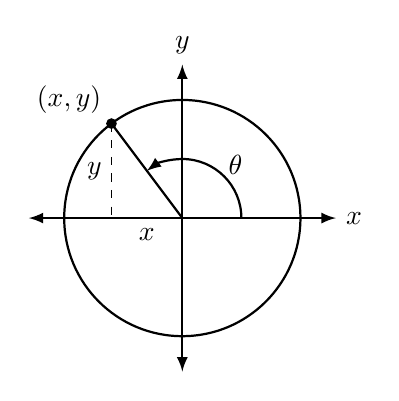
\begin{tikzpicture}[>=latex,scale=1.5,thick]
\draw [<->](-1.3,0)--(1.3,0) node [right] {$x$};
\draw [<->] (0,-1.3) -- (0,1.3) node [above] {$y$};
\draw (0,0) circle (1);
\draw [fill= black] (-.6,.8) circle (1pt);
\draw (0,0) -- (-.6,.8) node [above left] {$(x,y)$};
\draw [->] (.5,0) arc (0:127:.5);
\draw [dashed,thin] (-.6,.8) -- (-.6,0) node [pos=.5,left] {$y$};
\draw (-.3,0) node [below] {$x$};
\draw (.45,.45) node {$\theta$};
\end{tikzpicture}
\caption{ Measuring angles; reproduced from \apex\ Calculus, Version 3.0}\label{fig:measure_angle}
\end{figure}

Once we have swept over the angle we are interested in, we will need to know the x and y coordinates of the associated point on the circle. The x coordinate at the point is the value of $\cos{(\theta)}$ for that angle and the y coordinate is the value of $\sin{(\theta)}$ for that angle. The unit circle, shown in Figure \ref{fig:unitcircle}, shows these coordinates for a variety of common inputs. Here, the unit circle is shown with both angles measured in both degrees and radians, but remember that we are focusing on radians.

\begin{center}
\myincludegraphics{figures/figunitcircle}
	\captionsetup{type=figure}%
\caption{The unit circle; reproduced from \apex\ Calculus, Version 3.0}\label{fig:unitcircle}
\end{center}


Let's look at a few examples of how to use the unit circle to evaluate trigonometric functions. Remember, the unit circle will help us determine which x and y coordinates pair with each angle. The x coordinate gives us the value of cosine for the angle and the y coordinate gives us the value of sine for the angle.

\vskip \baselineskip

\example{ex_evaluating_trig}{Evaluating Trigonometric Functions}{Evaluate each of the following:

\noindent\begin{minipage}[t]{.5\textwidth}
		\begin{enumerate}
		\item	$\sin{(\frac{\pi}{4})}$	
		\item	$\tan{(\frac{\pi}{6})}$
		\item	$\sec{(3\pi)}$				
		\end{enumerate}
		\end{minipage}
		\begin{minipage}[t]{.5\textwidth}
		\begin{enumerate}\addtocounter{enumi}{3}
		\item	$\cos{(-\frac{3\pi}{4})}$	
		\item	$\csc{(\frac{2 \pi}{3})}$				
		\item	$\cot{(\frac{5 \pi}{6})}$	
		\end{enumerate}	
		\end{minipage}
}{Let's get started:

\begin{enumerate}
	\item Here, our input angle is $\frac{\pi}{4}$. This corresponds to the coordinate pair $(\frac{\sqrt{2}}{2}, \frac{\sqrt{2}}{2})$. We are interested in the value of sine, so we want to look at the y coordinate. This gives us 
			\begin{center}
		\begin{tabular}{| c |} \hline
			\\[-8pt]
			$\displaystyle \sin{\bigg(\frac{\pi}{4}\bigg)} = \frac{\sqrt{2}}{2}$ \\[-8pt]
			\\\hline
		\end{tabular}
	\end{center}
	\item Here, our input angle is $\frac{\pi}{6}$ which corresponds to the coordinate pair $(\frac{\sqrt{3}}{2}, \frac{1}{2})$. The coordinate pairs give us the values for cosine and sine, but doesn't directly give us a value for tangent, so we will need to use our definition of tangent. We have 
		\begin{equation*}
			\begin{split}
				\tan{\bigg(\frac{\pi}{6}\bigg)} &= \frac{\sin{(\frac{\pi}{6})}}{\cos{(\frac{\pi}{6})}} \\[6pt]
						      &=\frac{\frac{\sqrt{3}}{2}}{\frac{1}{2}} \\[6pt]
						      &= \frac{\sqrt{3}}{2} \times \frac{2}{1} \\[6pt]
						      & = \sqrt{3}
			\end{split}
	\end{equation*}
		So, our final answer is
\drawexampleline
			\begin{center}
		\begin{tabular}{| c |} \hline
			\\[-8pt]
			$\displaystyle \tan{\bigg(\frac{\pi}{6}\bigg)}= \sqrt{3}$ \\[-8pt]
			\\\hline
		\end{tabular}
	\end{center}
	\item Here, our input angle is $3\pi$. There is no angle labeled as $3\pi$ on the unit circle, so this one requires a bit more thought. We said earlier that the circle has $2\pi$ radians, so if we completely go around the circle, we have covered $2\pi$. We need to go another $3\pi-2\pi=\pi$ radians, so we can use the coordinates at $\pi$ radians to get our values for $3\pi$ radians. At $\pi$ radians, our coordinates are $(-1,0)$. This gives us:
		\begin{equation*}
			\begin{split}
				\sec{(3\pi)} & = \frac{1}{\cos{(3\pi)}} \\[6pt]
					     & = \frac{1}{-1} \\[6pt]
					     & = -1
			\end{split}
		\end{equation*}
		So, we have
			\begin{center}
		\begin{tabular}{| c |} \hline
			\\[-8pt]
			$\displaystyle \sec{(3\pi)}= -1$ \\[-8pt]
			\\\hline
		\end{tabular}
	\end{center}
	\item Here, our input angle is $-\frac{3\pi}{4}$. This means we are covering the unit circle by moving in a clockwise direction. We need to start at $0$ radians, and move $\frac{3\pi}{4}$ radians clockwise. This would put us at $\frac{5\pi}{4}$ radians. The coordinates are $(-\frac{\sqrt{2}}{2}, -\frac{\sqrt{2}}{2})$, so 
			\begin{center}
		\begin{tabular}{| c |} \hline
			\\[-8pt]
			$\displaystyle \cos{(-\frac{3\pi}{4})} = -\frac{\sqrt{2}}{2}$ \\[-8pt]
			\\\hline
		\end{tabular}
	\end{center}
\drawexampleline
	\item Here, our input angle is $\frac{2\pi}{3}$ radians, which gives coordinates of $(-\frac{1}{2}, \frac{\sqrt{3}}{2})$. Cosecant relies on sine, so we have
		\begin{equation*}
			\begin{split}
				\csc{\bigg(\frac{2\pi}{3}\bigg)} & = \frac{1}{\sin{(\frac{2\pi}{3})}} \\[6pt]
						       & = \frac{1}{\frac{\sqrt{3}}{2}} \\[6pt]
						       & = \frac{2}{\sqrt{3}} \\[6pt]
						       & = \frac{2}{\sqrt{3}} \times \frac{\sqrt{3}}{\sqrt{3}} \\[6pt]
						       & = \frac{2\sqrt{3}}{3}
			\end{split}
		\end{equation*}
		Notice that we rationalized the denominator. This means that we rewrote the fraction so that it would not have an irrational number, $\sqrt{3}$, in the denominator. This is a common last step in mathematics to standardize the form of the answer. Most answer keys will write the answer in the rationalized form, so it is a good habit to rationalize the denominator so that you can check your answers. Our final answer is
			\begin{center}
		\begin{tabular}{| c |} \hline
			\\[-8pt]
			$\displaystyle \csc{\bigg(\frac{2\pi}{3}\bigg)}= \frac{2\sqrt{3}}{3} $ \\[-8pt]
			\\\hline
		\end{tabular}
	\end{center}
	\item Here, we have an angle of $\frac{5\pi}{6}$, which has coordinates $(-\frac{\sqrt{3}}{2}, \frac{1}{2})$. This gives us
		\begin{equation*}
			\begin{split}
				\cot{\bigg( \frac{5\pi}{6}\bigg)} & = \frac{\cos{(\frac{5\pi}{6})}}{\sin{(\frac{5\pi}{6})}} \\
								  & = \frac{-\frac{\sqrt{3}}{2}}{\frac{1}{2}} \\
								  & = \frac{-\sqrt{3}}{2} \times \frac{2}{1} \\
								  & = -\sqrt{3}
			\end{split}
		\end{equation*}
			\begin{center}
		\begin{tabular}{| c |} \hline
			\\[-8pt]
			$\displaystyle \cot{\bigg( \frac{5\pi}{6}\bigg)} = -\sqrt{3}$ \\[-8pt]
			\\\hline
		\end{tabular}
	\end{center}
\end{enumerate}}\\

\vskip \baselineskip
\noindent\textbf{\large Properties of Trigonometric Functions}\\

Notice that on the unit circle, the values of the x and y coordinates range between -1 and 1. Since these are the output values of the sine and cosine functions, we say that the \emph{range}, or the output values, of sine and cosine is $[-1,1]$, meaning that the output can get as small as -1 and as large as 1. Additionally, sine and cosine are defined for any input value, so for each the domain is $(-\infty,\infty)$.

The other four trigonometric functions are all defined in terms of sine and cosine, where either sine or cosine is in the denominator of a fraction. This means that the domains of these functions are limited. Both secant and tangent have cosine in the denominator, meaning that they will be undefined anytime cosine is 0. Cosine is 0 at the odd multiples of $\frac{\pi}{2}$. This tells us that these odd multiple of $\frac{\pi}{2}$, values like $-\frac{3\pi}{2}$, $-\frac{\pi}{2}$, $\frac{\pi}{2}$, and $\frac{3\pi}{2}$ are not part of the domain for tangent or for secant. Like sine and cosine, the output values of secant is limited; its range is $(-\infty,-1]\cup [1,\infty)$, but the range for tangent is not limited; its range is $(-\infty,\infty)$.

Cosecant and cotangent both have sine in the denominator for their definitions; this means they are undefined whenever sine is 0. Sine is 0 at the integer multiples of $\pi$: $-5\pi$, $-3\pi$, $-\pi$, $\pi$, $3\pi$, etc. As with secant, the output values of cosecant are limited so its range is also $(-\infty,-1] \cup [1,\infty)$; the range of cotangent is not limited and is $(-\infty,\infty)$.




\printexercises{exercises/intro_trig_exercises}


%\clearpage
